%\author{traduit par J\'er\'emy Garniaux}

% vim: set textwidth=78 autoindent:

\section{Les extensions de QGIS}\label{sec:extensions}\index{extensions}

% when the revision of a section has been finalized, 
% comment out the following line:
%\updatedisclaimer

%QGIS has been designed with a plugin architecture.
%This allows new features/functions to be easily added to the application.
%Many of the features in QGIS are actually implemented as \textbf{core} or \textbf{external} plugins.\index{plugins!types} 

QGIS repose sur un syst\`eme d'extensions.
Ce dernier permet d'ajouter facilement de nouvelles fonctions au logiciel. 
De nombreuses nouvelles fonctions de QGIS sont impl\'ement\'ees comme des extensions \textbf{principales} ou \textbf{compl\'ementaires}. \index{plugins!types} 

%\begin{itemize}
%\item \textbf{Core Plugins} are maintained by the QGIS Development Team and are automatically part of every QGIS distribution.
%They are written in one of two languages: C++ or Python.
%More information about core plugins are provided in Section \ref{sec:core_plugins}.
%\item \textbf{External Plugins} are currently all written in Python.
%They are stored in external repositories and maintained by the individual author.
%They can be added to QGIS using the core plugin called \filename{Plugin Installer}.
%More information about external plugins are provided in Section \ref{sec:external_plugins}.
%\end{itemize}

\begin{itemize}
\item Les \textbf{extensions principales} sont maintenues par l'\'equipe de d\'eveloppement de QGIS et sont int\'egr\'ees automatiquement \`a chaque nouvelle distribution de QGIS.
Elles sont \'ecrites en C++ ou en Python.
On trouvera plus d'informations sur les extensions principales dans la Section \ref{sec:core_plugins}.
\item Les \textbf{extensions compl\'ementaires} sont actuellement toutes \'ecrites en Python.
Elles sont stock\'ees dans des d\'ep\^ots externes et maintenues par leurs auteurs.
Elles peuvent \^etre ajout\'ees \`a QGIS en utilisant l'extension principale nomm\'ee \filename{Gestionnaire d'extensions}.
On trouvera plus d'informations sur les extensions compl\'ementaires dans la Section \ref{sec:external_plugins}.
\end{itemize}

%\subsection{Managing Plugins}\label{sec:managing_plugins}
%\index{plugins!managing} 
%
%Managing plugins in general means loading or unloading them using the \filename{Plugin Manager} plugin.
%External plugins need to be first installed using the \filename{Plugin Installer} plugin.

\subsection{G\'erer les extensions}\label{sec:managing_plugins}
\index{plugins!managing} 

De mani\`ere g\'en\'erale, g\'erer les extensions consiste \`a les afficher ou pas \`a l'aide du \filename{Gestionnaire d'extension}.
Les extensions compl\'ementaires doivent d'abord \^etre install\'ees \`a l'aide du \filename{Gestionnaire d'extension}.

%\subsubsection{Loading a QGIS Core Plugin}\label{sec:load_core_plugin} 

%Loading a QGIS Core Plugin is provided in the main menu \mainmenuopt{Plugins} > \dropmenuopttwo{mActionShowPluginManager}{Manage Plugins...}.\index{plugins!manager}

%\begin{figure}[ht]
%   \begin{center}
%   \caption{Plugin Manager \nixcaption}\label{fig:pluginmanager}\smallskip
%   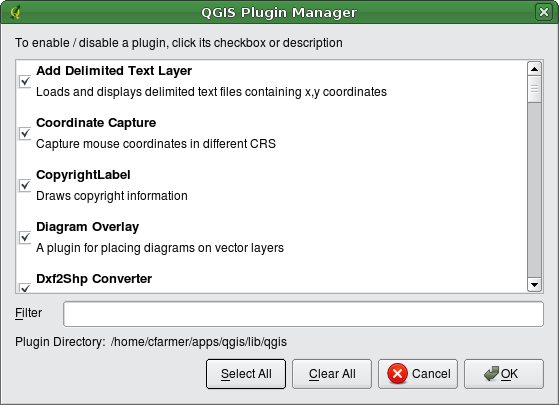
\includegraphics[clip=true, width=14cm]{pluginmanager}
%\end{center}
%\end{figure}

%The Plugin Manager lists all the available plugins and their status (loaded or unloaded).
%All available means all core plugins and all external plugins you added using \filename{Plugin Installer} plugin (see Section \ref{sec:external_plugins}). 
%Figure \ref{fig:pluginmanager} shows the Plugin Manager dialog.
%Loaded plugins are "remembered" when you exit the application and restored the next time you run QGIS.

%\begin{Tip}\caption{\textsc{Crashing Plugins}}\index{crashes}
%\qgistip{If you find that QGIS crashes on startup, a plugin may be at fault.
%You can stop all plugins from loading by editing your stored settings file (see \ref{subsec:gui_options} for location).
%Locate the plugins settings and change all the plugin values to false to prevent them from loading.
%\nix {For example, to prevent the Delimited text plugin from loading, the entry in \$HOME/.config/QuantumGIS/qgis.conf on Linux should look like this:\usertext{Add %Delimited Text Layer=false}.}
%\normalfont 
%Do this for each plugin in the [Plugins] section.
%You can then start QGIS and add the plugins one at a time from the Plugin Manger to determine which is causing the problem.}
%\end{Tip} 

\subsubsection{Installer une extension principale}\label{sec:load_core_plugin} 

On installe une extension principale \`a l'aide du menu \mainmenuopt{Plugins} > \dropmenuopttwo{mActionShowPluginManager}{Gestionnaire d'extension...}.\index{plugins!manager}

\begin{figure}[ht]
   \begin{center}
   \caption{Gestionnaire d'extension \nixcaption}\label{fig:pluginmanager}\smallskip
   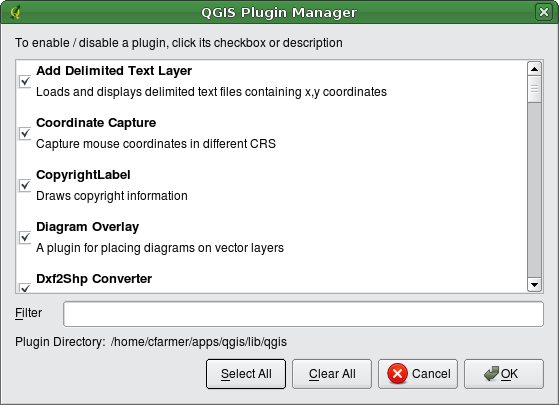
\includegraphics[clip=true, width=14cm]{pluginmanager}
\end{center}
\end{figure}

Le gestionnaire d'extension liste toutes les extensions disponibles et leur statut (install\'e ou pas).
"Tous disponibles" signifie que toutes les extensions principales ou compl\'ementaires que vous avez ajout\'ees \`a l'aide de l'extension \filename{Gestionnaire d'Extension} (see Section \ref{sec:external_plugins}). 
La figure \ref{fig:pluginmanager} montre la bo\^ite de dialogue du Gestionnaire d'extension.
Les extensions install\'ees sont m\'emoris\'ees lorsque vous quittez l'application et seront restaur\'ees \`a la prochaine ouverture de QGIS.

\begin{Astuce}\caption{\textsc{Extensions et plantages}}\index{crashes}
\qgistip{Si votre installation de QGIS plante au d\'emarrage, une extension est peut-\^etre en cause.
Vous pouvez \'eviter le chargement des extensions en \'editant votre fichier de configuration (voir \ref{subsec:gui_options} pour localiser ce fichier).
Localisez la configuration de l'extension et changez toutes les valeurs \`a "false" pour emp\^echer leur chargement.
\nix Par exemple, pour \'eviter le chargement de l'extension "Ajouter une couche texte d\'elimit\'ee", l'entr\'ee de \$HOME/.config/QuantumGIS/qgis.conf doit ressembler \`a \usertext{Add Delimited Text Layer=false}.
\normalfont 
Faites de m\^eme pour chaque extension dans la section [Extension].
Vous pouvez ensuite d\'emarrer QGIS et ajouter les extensions une \`a la fois depuis le Gestionnaire d'extension pour d\'eterminer celle qui est la source du probl\`eme.}
\end{Astuce}

%\subsubsection{Loading an external QGIS Plugin}\label{sec:load_external_plugin} 

%To be able to integrate external plugins into QGIS you first need to load the \filename{Plugin Installer} plugin as desribed in Section \ref{sec:load_core_plugin}.
%Then you can load external QGIS python plugin in two steps: 

%\begin{enumerate}
%\item Download an external plugin from a repository using the \filename{Plugin Installer} (Section \ref{sec:python_plugin_installer}).
%The new external plugin will be integrated into the list of available plugins in the \filename{Plugin Manager}.
%\item Load the plugin using the \filename{Plugin Manager}.
%\end{enumerate}

\subsubsection{Installer une extension compl\'ementaire de QGIS}\label{sec:load_external_plugin} 

Afin de pouvoir int\'egrer des extensions compl\'ementaires dans QGIS, vous devez d'abord installer l'extension \filename{Gestionnaire d'extension} comme d\'ecrit dans la Section \ref{sec:load_external_plugin}.
Les extensions python compl\'ementaires peuvent ensuite \^etre install\'ees en deux \'etapes :

\begin{enumerate}
\item T\'elechargez une extension compl\'ementaire depuis un d\'ep\^ot \`a l'aide de l'\filename{Installeur d'extension python} (Section \ref{sec:python_plugin_installer}).
La nouvelle extension compl\'ementaire sera int\'egr\'ee dans la liste des extensions disponibles du \filename{Gestionnaire d'extension}.
\item Installez l'extension \`a l'aide du \filename{Gestionnaire d'extension}.
\end{enumerate}

%\subsubsection{Using the QGIS Python Plugin Installer}\index{plugins!installing}\label{sec:python_plugin_installer}
%\index{plugins!Python Plugin Installer}\index{plugins!upgrading}

%\begin{figure}[ht]
%   \begin{center}
%   \caption{Installing external python plugins \nixcaption}
%\label{fig:plugininstaller}\smallskip
%   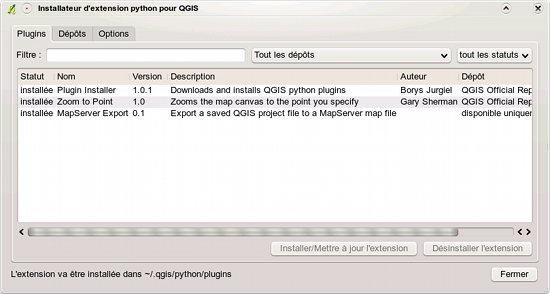
\includegraphics[clip=true, width=14cm]{plugininstaller}
%\end{center}
%\end{figure}

\subsubsection{Utiliser l'installeur d'extension python de QGIS}\index{plugins!installing}\label{sec:python_plugin_installer}
\index{plugins!Python Plugin Installer}\index{plugins!upgrading}

\begin{figure}[ht]
   \begin{center}
   \caption{Installer des extensions compl\'ementaires python\nixcaption}
\label{fig:plugininstaller}\smallskip
   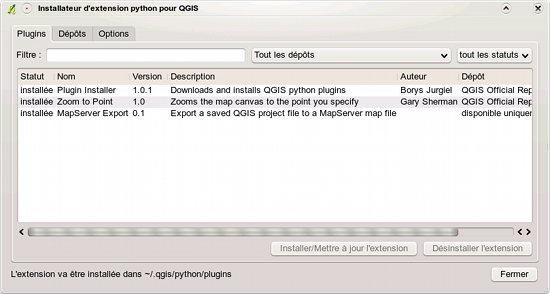
\includegraphics[clip=true, width=14cm]{plugininstaller}
\end{center}
\end{figure}

%In order to download and install an external Python plugin, click the menu \mainmenuopt{Plugins} > \dropmenuopttwo{plugin_installer}{Fetch Python Plugins...}.
%The \filename{Plugin Installer} window will appear (figure \ref{fig:plugininstaller}) with the tab \tab{Plugins}, containing the list of all Python plugins available in remote repositories as well as installed ones. Each plugin can be either:
%\begin{itemize}
%\item \textbf{not installed} - it means the plugin is available in the repository, but is not installed yet. In order to install, select it from the list and click the \button{Install plugin} button.
%\item \textbf{new} - the same as before but the plugin is seen for the first time.
%\item \textbf{installed} - the plugin is installed. If it's also available in any repository the \button{Reinstall plugin} button is enabled. But if the available version is older than the installed one, the \button{Downgrade plugin} button appears instead.
%\item \textbf{upgradeable} - the plugin is installed, but there is an updated version available. The \button{Upgrade plugin} button is enabled.
%\item \textbf{invalid} - the plugin is installed, but is unworkable. The reason is explained in the plugin description.
%\end{itemize}

Pour t\'el\'echarger et installer une extension python compl\'ementaire, cliquez  sur le menu \mainmenuopt{Plugins} > \dropmenuopttwo{plugin_installer}{R\'ecup\'eration des extensions python...}.
La fen\^etre de l'\filename{Installeur d'extension python} appara\^itra (figure \ref{fig:plugininstaller}) avec l'onglet \tab{Plugins}, qui pr\'esente la liste de toutes les extensions python install\'ees ou disponibles dans des d\'ep\^ots distants. Chaque extension peut-\^etre soit :
\begin{itemize}
\item \textbf{non install\'ee} - signifie que l'extension est disponible dans le d\'ep\^ot, mais n'est pas encore install\'ee. Pour l'installer, s\'electionnez-la dans la liste et cliquez sur le bouton \button{Installer l'extension}.
\item \textbf{nouveau} - m\^eme statut que ci-dessus, mais l'extension appara\^it pour la premi\`ere fois.
\item \textbf{install\'ee} - l'extension est install\'ee. Si elle est \'egalement disponible dans un d\'ep\^ot, le bouton \button{R\'e-installer l'extension} est actif. En revanche, si la version disponible est plus ancienne que la version install\'ee, le bouton \button{???} appara\^it \`a la place.
\item \textbf{mise \`a jour} - l'extension est install\'ee, mais une version plus r\'ecente est disponible, le bouton \button{Mise \`a jour de l'extension} est actif.
\item \textbf{invalide} - l'extension est install\'ee, mais ne fonctionne pas. Les d\'etails sont donn\'es dans la description de l'extension.
\end{itemize}

%\minisec{Plugins tab}
%
%To install a plugin, select it from the list and click the \button{Install plugin} button. The plugin is installed in its own directory, e.g. for \nix under \filename{\$HOME/.qgis/python/plugins} and is only visible for the user who has installed it. See a list of other OS specific subdirectory used for plugins in Section~\ref{subsec:pyfoursteps}. If the installation is successful, a confirmation message will appear. Then you need go to the \mainmenuopt{Plugins} > \dropmenuopttwo{mActionShowPluginManager}{Manage Plugins...} and load the installed plugin. 
%
%If the installation fails, the reason is displayed. The most often troubles are related to connection errors and missing Python modules. In the former case you'll probably need to wait some minutes or hours, in the latter one you need to install the missing modules in your operating system prior to using the plugin. \nix{For Linux, most required modules should be available in a package manager}. \win{For install instructions in Windows visit the module home page}. If you use a proxy, you may need to configure it under the menu \mainmenuopt{Settings} > \dropmenuopttwo{mActionOptions}{Options} on the \tab{Proxy} tab.
%
%The \button{Uninstall plugin} button is enabled only if the selected plugin is installed and it's not a core plugin. Note that if you have installed an update of a core plugin, you can still uninstall this update with the \button{Uninstall plugin} and revert to the version shipped within Quantum GIS install package. This one cannot be uninstalled.

\minisec{Onglet Plugins}

Pour installer une extension, s\'electionnez-la dans la liste et cliquez sur le bouton \button{Installer l'extension}. L'extension est install\'ee dans son propre r\'epertoire, par ex. pour \nix dans \filename{\$HOME/.qgis/python/plugins} et n'est visible que pour l'utilisateur qui l'a install\'ee. Voir une liste des r\'epertoires d'installation des extensions sous d'autres OS dans la Section~\ref{subsec:pyfoursteps}. Si l'installation r\'eussit, un message de confirmation appara\^it. Cliquez ensuite sur le menu \mainmenuopt{Plugins} > \dropmenuopttwo{mActionShowPluginManager}{Gestionnaire d'extension...} et chargez l'extension fra\^ichement install\'ee.
and load the installed plugin.

Si l'installation ne fonctionne pas, la raison est indiqu\'ee. Les probl\`emes les plus fr\'equents sont dus \`a des erreurs de connexion et \`a des modules Python manquants. Dans le premier cas, il vous faudra probablement attendre quelques minutes ou heures ; dans le second cas, il sera n\'ecessaire d'installer les modules manquants avant d'utiliser les extensions. \nix{Pour Linux, les modules les plus recherch\'es devraient \^etre disponibles dans un gestionnaire de paquets}. \win{Pour des installations d'instruction dans Windows, visitez la page web du module}. Si vous utilisez un proxy, vous pourrez avoir besoin de le configurer dans le menu \mainmenuopt{Pr\'ef\'erences} > \dropmenuopttwo{mActionOptions}{Options} dans l'onglet \tab{Proxy}.

Le bouton \button{D\'esinstaller l'extension} est actif seulement si l'extension s\'electionn\'ee est install\'ee et n'est pas une extension principale. Notez que si vous avez install\'e une mise \`a jour d'une extension principale, il est toujours possible de d\'esinstaller cette mise \`a jour avec le bouton \button{D\'esinstaller l'extension} et revenir \`a la version d'origine fournie \`a l'installation de Quantum GIS. Cette derni\`ere ne peut pas \^etre d\'esinstall\'ee.

%\minisec{Repositories tab}
%
%The second tab \tab{Repositories} contains a list of plugin repositories available for the Plugin Installer. By default, only the QGIS Official Repository is used. You can add some user-contributed repositories, including the central QGIS Contributed Repository and a few author repositories by clicking the \button{Add 3rd party repositories} button. Those repositories contain a huge number of more or less useful plugins but please note that they aren't maintained by the QGIS Development Team and we can't take any responsibility for them. You can also manage the repository list manually, that is add, remove and edit the entries. Temporary disabling a particular repository is possible clicking the \button{Edit...} button.
%
%The \checkbox{Check for updates on startup} checkbox makes QGIS looking for plugin updates and news. If it's enabled, all repositories listed and enabled on the \tab{Repositories} tab are checked whenever the program is starting. If a new plugin or an update for one of installed plugins is available, a clickable notification appears in the Status Bar. If the checkbox is disabled, looking for updates and news is performed only when Plugin Installer is being launched from the menu.
%
%In case of some internet connection problems a \textit{Looking for new plugins...} indicator in the Status Bar may stay visible during whole QGIS session and cause a program crash when exiting. In this case please disable the checkbox.

\minisec{Onglet D\'ep\^ots}

Le second onglet \tab{D\'ep\^ots} contient une liste de d\'ep\^ots d'extensions disponibles. Par d\'efaut, seul le d\'ep\^ot officiel de QGIS (QGIS Official Repository) est utilis\'e. Vous pouvez ajouter des d\'ep\^ots contenant des contributions d'utilisateurs, notamment le d\'ep\^ot de contributions de QGIS (QGIS Contributed Repository) et quelques d\'ep\^ots d'auteurs en cliquant sur le bouton \button{Ajouter un d\'ep\^ot-tiers d'extension \`a la liste}. Ces d\'ep\^ots contiennent une grande quantit\'e d'extensions plus ou moins utiles, mais veuillez noter qu'elles ne sont pas maintenues par l'\'equipe de d\'eveloppement de QGIS et que nous ne pouvons prendre aucune responsabilit\'e pour elles. Vous pouvez \'egalement g\'erer la liste de d\'ep\^ots manuellement, pour ajouter, retirer ou \'editer des entr\'ees. D\'esactiver temporairement un d\'ep\^ot particulier est possible en cliquant sur le bouton \button{Editer}.


La case \checkbox{Chercher des mises \`a jour au d\'emarrage} configure QGIS pour rechercher des mises \`a jour et des actualit\'es relatives aux extensions. Si la case est coch\'ee, tous les d\'ep\^ots list\'es et activ\'es dans l'onglet \tab{D\'ep\^ots} sont v\'erifi\'es \`a chaque d\'emarrage du programme. Si une nouvelle extension ou une mise \`a jour pour une des extensions install\'ees est disponible, une notification cliquable appara\^it dans la barre de statut. Si la case est d\'ecoch\'ee, la recherche de mises \`a jour et d'actualit\'es s'effectue uniquement lorsque l'Installeur d'Extension est lanc\'e manuellement depuis le menu.

En cas de probl\`emes de connexion Internet, un indicateur \textit{Recherche de nouvelles extensions...} dans la barre de statut peut rester visible durant toute la session QGIS et faire planter le programme \`a la fermeture. Dans ce cas, d\'ecochez la case.

%\subsection{Data Providers}\index{data providers}
%
%Data Providers are "special" plugins that provides access to a data store.
%By default, QGIS supports PostGIS layers and disk-based data stores supported by the GDAL/OGR library (Appendix \ref{appdx_ogr}).
%A Data Provider plugin extends the ability of QGIS to use other data sources.
%
%Data Provider plugins are registered automatically by QGIS at startup.
%They are not managed by the Plugin Manager but used behind the scenes when a data type is added as a layer in QGIS.

\subsection{Fournisseurs de donn\'ees}\index{data providers}

Les Fournisseurs de donn\'ees sont des extensions "sp\'eciales" donnant acc\`es \`a un d\'ep\^ot de donn\'ees.
Par d\'efaut, QGIS supporte les couches PostGIS et les bases de donn\'ees fichiers couverts par la biblioth\`eque GDAL/OGR(Appendix \ref{appdx_ogr}).
L'utilisation d'extensions pour fournir des donn\'ees permet d'\'elargir les sources de donn\'ees utilisables par QGIS.

Les extensions fournissant des donn\'ees sont automatiquement enregistr\'ees par QGIS au d\'emarrage.
Elles ne sont pas g\'er\'ees par le Gestionnaire d'Extension, mais utilis\'ees en arri\`ere-plan lorsqu'un type de donn\'ees est ajout\'e comme couche dans QGIS.
